\chapter{Исследовательская часть}

\section{Формализация объекта и его признака}
\label{formal}
Согласно согласованному варианту, формализуем объект <<время в пути от дома до вуза>> следующим образом: определим числовой признак объекта, на основании которого составим набор термов.

Согласно варианту, признаком, по которому будет производиться поиск объектов, будет являться время в минутах --- целое число.

Определим следующие термы, соответствующие признаку <<время>>:
\begin{enumerate}[label=\arabic*), itemindent=1em]
	\item <<Очень долго>>;
	\item <<Долго>>;
	\item <<Нормально>>;
	\item <<Близко>>;
	\item <<Очень близко>>.
\end{enumerate}

Также введём числовое множество множество, описывающее термы:
\begin{equation}
	\label{eq:h}
	H = \{10, 20, 30, 40, 50,60,70,80,90,100,110,120\}
\end{equation}
\newpage
\section{Анкетирование респондентов}

Было проведено анкетирование следующих респондентов:
\begin{enumerate}[label=\arabic*), itemindent=1em]
	\item Светличная Алина --- Респондент 1;
	\item Марченко Владислав --- Респондент 2;
	\item Царев Антон --- Респондент 3;
	\item Лагутин Даниил --- Респондент 4;
\end{enumerate}

Респонденты, выступающие в качестве экспертов, для каждого из приведённых выше термов указали соответствующий промежуток, элементами которого являются числа из введённого для поставленной задачи множества оценимоемой величины.

Результаты анкетирования перечисленных респондентов продемонстрированы в таблице~\ref{tbl:anket}. В данной таблице Респ. --- сокращение от <<Респондент>>.

\begin{center}
	\begin{threeparttable}
			\caption{Результаты анкетирования}
		\label{tbl:anket}
	\begin{tabular}{|c|c|c|c|c|}\hline
		Терм & Респ. 1 & Респ. 2 & Респ. 3  & Респ. 4 \\ \hline
		1 & 90--120  &80--120  & 100--120 & 80--120\\ \hline 
		2 & 50--90  &  60--80  & 80--100& 60--80\\ \hline
		3&  30--50  & 40--60   &50--80 &  40--60 \\ \hline
		4 &  20--30 & 30--40  & 30--50 & 20--40 \\ \hline
		5 & 10--20    & 10--30 &10--30 &10--20  \\ \hline
\end{tabular}	
\end{threeparttable}
\end{center}

\section{Функция принадлежности термам}

Графики функций принадлежности числовых значений временным термам, приведён на рис. \ref{img:graph_sorted}.
\begin{center}
	\centering{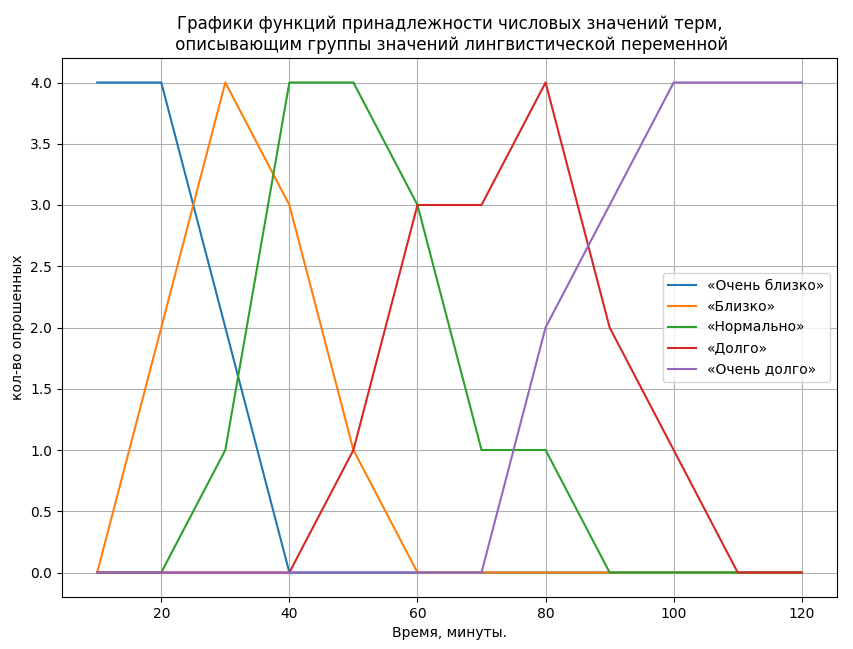
\includegraphics[trim=0 0 0 -5cm bb=0 0 800 800, scale=0.75]{src/good}}
	\captionof{figure}{Зависимость словесной оценки респондентов от количества
		минут, потраченных на дорогу от дома до вуза}
	\label{img:graph_sorted}
\end{center}

\section{Вывод}
По полученным результатам иследования можно сделать вывод, что 
